\chapter{Spektrale Methoden\label{chapter:klima}}
\lhead{Spektrale Methoden}
\begin{refsection}
\chapterauthor{Peter Nötzli}



\section{Einleitung
\label{klima:einleitung}}
\rhead{Einleitung}

\begin{figure}
\centering
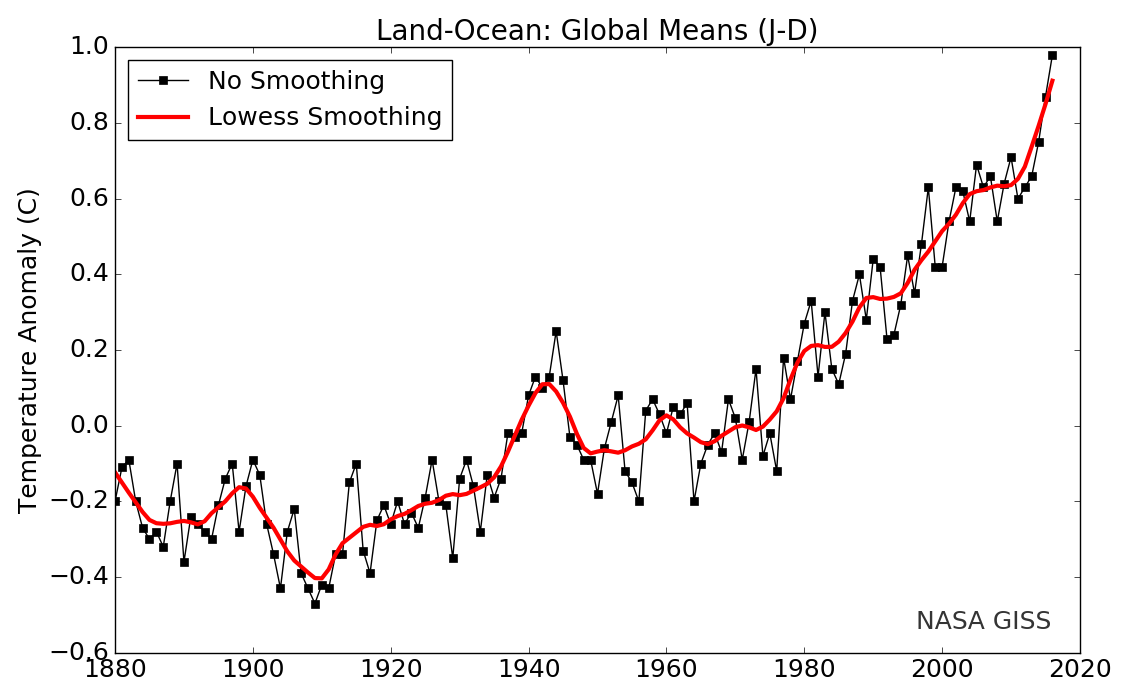
\includegraphics[width=\hsize]{klima/nasa_giss.png}
\caption{Grafik der globalen Jahresmitteltemperaturen seit 1880. Quelle: National Aeronautics and Space Administration Goddard Institute for Space Studies kurz NASA GISS \url{https://data.giss.nasa.gov/gistemp/graphs/customize.html}.
\label{klima:einleitung:nasa}}
\end{figure}

Die Klimaerwärmung schreitet voran, gleichzeitig, oder gerade deswegen kommen in der Gesellschaft dazu immer mehr Fragen auf. Gibt es eine Klimaerwärmung? Wie entwickelt sich diese? Was bedeutet dies für uns? Betrifft es mich überhaupt? Die erste und wohl einfachste Frage vorweg, ja es gibt die Klimaerwärmung. Dies ist deutlich zu erkennnen wenn wir die globale Temperaturentwicklung seit 1880 bis heute betrachten (Abbildung~\ref{klima:einleitung:nasa}). Diese Frage ist deshalb einfach zu beantworten, da diese nach einer Entwicklung frägt welche bereits, oder zumindest teilweise, in der Vergangeheit liegt. Die Auswirkungen dieser Entwicklung und wie weit diese noch fortschreitten wird sind Dinge, welche in der Zukunft liegen. Somit kann für die restlichen Fragen und auch viele der nicht gestellten Fragen keine pauschale Antwort gegeben werden. Obwohl eine Tendenz der Temperaturentwicklung erkennbar ist, diese mit ein bisschen Gefühl weiter zu führen und abzuschätzen kann wohl nicht richtig sein, da es sämtliche Faktoren welche einen Einfluss auf das Klima haben ignoriert. Da wir dennoch gerne wissen wollen welche Einflüsse welche Auswirkungen haben und wir auch nicht warten möchtenx bis es bereits zu spät ist, müssen wir auf Klimamodelle zurückgreifen. Wie so ein Klimamodell ausschauen könnte und wie es aufgebaut sein kann soll in diesem Kapitel aufgezeigt werden.



\section{Geschichte der Numerischen Strömungsmechanik
\label{section:klima:geschichte}}
\rhead{Geschichte}
Die numerische Strömungsmechanik, heute auch als CFD bekannt (Computational Fluid Dynamics) bezeichnet eine etablierte Methode, um verschiedenste Problemstellungen der Strömungsmechanik approximativ mit numerischen Modellen zu lösen. Die Validierung der Methoden erfolgt durch den Vergleich mit quantitativen Experimenten.



\subsection{Entstehung der Wettervorhersagen
\label{subsection:klima:wetter}}
Am Anfgang war das Wetter. Dann kam der Mensch und wollte wissen, wie das Wetter in Zukunft sein wird. Dies aus verschiedensten Gründen so wollen wir heute gerne wissen, welches Wetter am Wochenende ist, damit wir bereits anfangs Woche einen Ausflug organisieren können.

Bedeutung hatten Wettervorhersagen, früher wie heute, so kann eine Wettervorhersage wesentlichen Einfluss auf das Ernteglück haben. So entstanden schon früh sogenannte Bauernregeln, diese gingen meist davon aus dass sich das Wetter aufgrund Wetterereignissen an bestimmten Tagen in eine gewisse Richtung entwickeln. Die Korrektheit solcher Aussagen sind wohl eher Zufälle als korrekte Vorhersagen, so sind es eher die ähnlichen Wetterverhältnisse der jeweiligen Jahreszeit welche solch eine Regel von Zeit zu Zeit als korrekt erscheinen lässt. Jedoch waren verschiedenste Naturphänomene bereits bekannt, als Beispiel die Silberdiestel, auch als Wetterdiestel bekannt, welche seine Blütenblätter bei erhöhter Luftfeuchtigkeit aufrollt und so vor nahendem Regen warnen kann.1660 erkannte Otto von Guericke erstmals den Zusammenhang zwischen abfallendem Luftdruck und dem Aufziehen eines Unwetters.

Anfangs des 19. Jahrhunderts entstanden in Europa die ersten Wetterstationen, es waren jedoch noch keine Wettervorhersagen möglich. Dies aus dem einfachen Grund, da sich das Wetter schneller in eine nahende Stadt bewegen konnte als man die Daten dort hinbringen hätte können.

1835 konnte mit dem aufkommen der Telegrafie dieses Problem gelöst werden, erstmals waren einfache Prognosen möglich. Diese reichten oft nur einzelne Tage in die Zukunft und waren lokal begrenzt. Die Genauigkeit dieser ist nicht mit heutigen Massstäben vergleichbar.

Vilhelm Bjerknes (1862-1951) war der erste, welcher erkannte dass die Problemstellung der Wettervorhesage sich aus Physik und Mathematik zusammensetzt. Im wesentlichen stellte er fest, dass für die Berechnung der Strömung der Atmosphäre genaue Kenntnisse der Grundgesetze und der Anfangsbestimmungen notwendig und ausreichend für eine Wettervorhersage sind.



\subsection{Lewis Fry Richardson
\label{subsection:klima:richardson}}

\begin{figure}
\centering
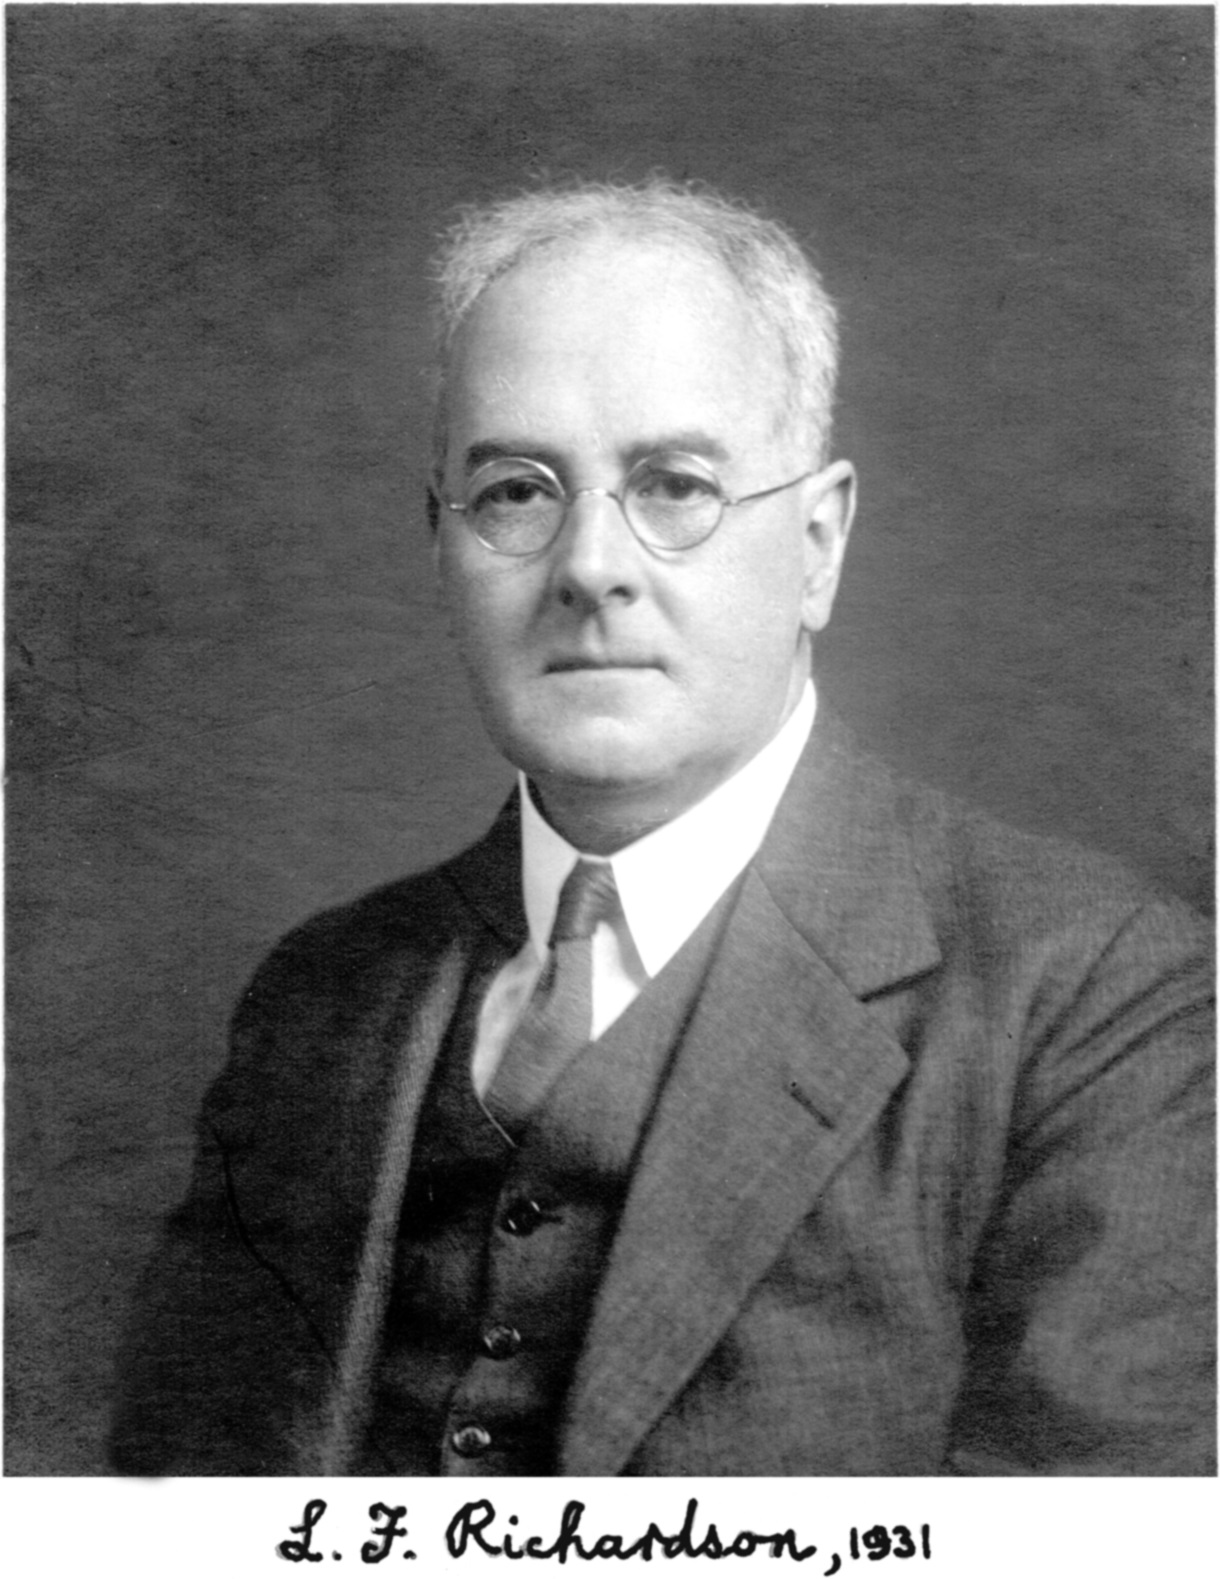
\includegraphics{klima/richardson.jpg}
\caption{Lewis Fry Richardson \cite{klima:biography}
\label{klima:geschichte:richardson}}
\end{figure}

Lewis Fry Richardson (1881-1953) Abbildung~\ref{klima:geschichte:richardson} veröffentlichte 1922 seine Arbeit mit dem Titel {\em Weather Prediction by Numerical Process}, in welcher er die erste numerische Wettervorhersage tätigte. Für seine Berechnungen, die er um 1917 durchführte, verwendete er Druck- und Temperatur-Daten verschiedenster Stationen in Europa. Er legte für seine Berechnung ein Gitter über Europa, dieses hatte eine Breite von 2°89' und eine Länge von 1°80', und 5 vertikale Layer. Dies entspricht in etwa einer Abmessung von 320km mal 200km je Feld und umfasst ingesamt etwa 150 Punkte an welchen die Drucktendenz berechnet werden sollte. Er verwendete dabei die horizontalen Impulserhaltungsgleichungen, die ideale Gasgleichung und die Kontinuitätsgleichung \eqref{skript:speziell:kontinuitaetsgleichung} (diese wurde auf Seite \pageref{skript:speziell:kontinuitaetsgleichung} bereits behandelt). Die Vorhersage für 24 Stunden bedeutete dabei einen Rechenaufwand von 3 Monaten. Im wesentlichen basierte die Berechnung auf einer Unterteilung in die einzelnen Zellen welche jeweils mit 7 Werten befüllt waren. Dies waren der Luftdruck, Temperatur, Dichte, Luftfeuchtigkeit und den Volumenströmen richtung Norden, Osten und Aufwärts.

Die erste Berechnung von Richardson lieferte dann auch ein Resultat, welches einen Druckabfall von 145mbar in 6h voraussagte. Eine solch grosse Veränderung ist absolut unrealistisch und nicht einmal im Zentrum eines Sturmtiefes möglich. Das Problem war, dass die Daten des Boden-Drucks, welche als Anfangsbedinungen verwendet wurden, Fehler enthielten. Diese Fehler führten dazu, dass sich während der numerischen Prozedur die Werte aufschaukelten und somit zu hohen Drucktendenzen führten. (Eine Berechnung aufgrund der selben Beobachtungsdaten, die jedoch zu Beginn gefiltert werden, führt mit Richardson's Algorithmus zu plausiblen Vorhersagen, 3.2 mbar in 6h \cite{klima:stocker}).

Dies zeigt exemplarisch wie heikel die Anfangsbedingungen von Wetter- und Klimamodellen sich auf das Ergebniss auswirken können. Jedoch hätten selbst die besten Initialisierungswerte zu einer Instabilität geführt und eine Resultat für grosse Vorhersagezeiten verunmöglicht. Erst durch die Verfügbarkeit erster Computer in den 40er Jahren wurde Richardsons Arbeit zur  Wettervorhersage praktikabel und wurde gegen Ende des 2. Weltkriegs als taktisches Mittel eingesetzt.

\begin{figure}
\centering
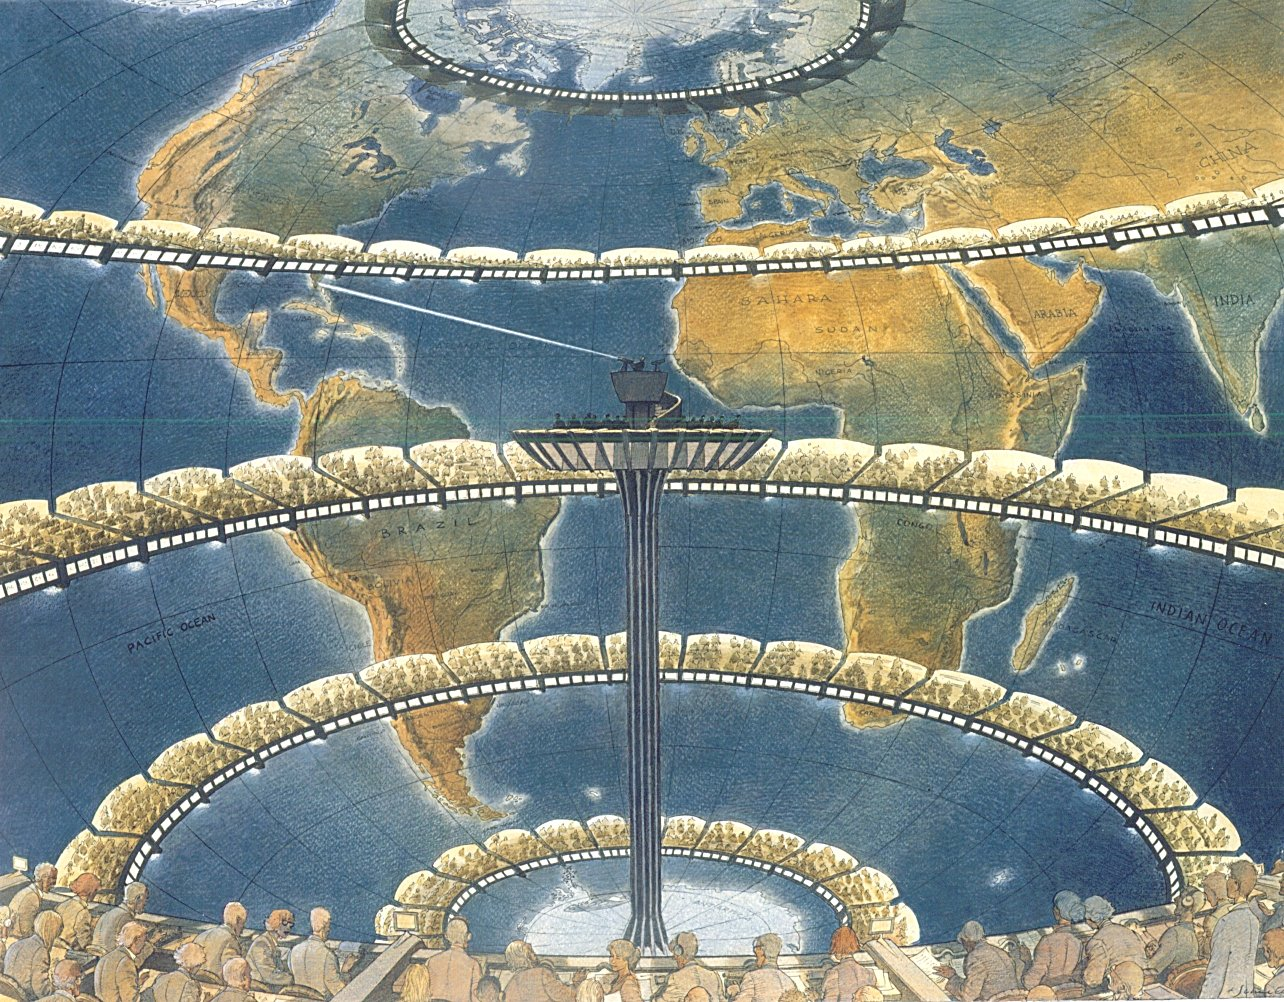
\includegraphics{klima/64000.jpg}
\caption{Interpretation eines Künstlers von Richardsons Vorhersage Fabrik \cite{klima:biography}
\label{klima:geschichte:richardson}}
\end{figure}

Richardson äusserte in seiner Arbeit die Idee einer Vorhersage Fabrik in welcher er mit 64'000 Rechnern (damit waren damals noch Menschen gemeint), welche gleichzeitig Berechnungen durchführten und zum weiterrechnen jeweils die Werte ihrer Nachbarzellen übernehmen sollten, das Wetter für den ganzen Planeten berechnen könnte. Diese Idee wurde vom Künstler François Schuiten in der Abbildung~\ref{klima:geschichte:richardson} versinnbildlicht.

Zudem äusserte Richardson einen weiteren Traum:
\begin{quote}
Perhaps some day in the dim future it will be possible to advance the computations faster than the weather advances....
\end{quote}
Von diesem wissen wir, dass es heute nicht nur möglich ist, sondern werden mit jeden neuen Wettervorhersage daran erinnert, dass dies an jedem Tag aufs neue geschieht.



\subsection{Wettervorhersagen in der Schweiz
\label{section:klima:wettervorhersagen}}
\rhead{Wettervorhersagen}

Insgesamt haben wir in der Schweiz 7 private Wetterdienst-Anbieter und den Bundesbetrieb MeteoSchweiz. In diesem Abschnitt wird mehrheitlich auf MeteoSchweiz und deren Methoden eingegangen, dies weil MetheoSchweiz ihre Methoden im Internet öffentlich einsehbar teilen.

MeteoSchweiz betreibt mit SwissMetNet ein eigenes automatisches Messnetz welches ca.160 Station umfässt. Diese liefern alle 10min aktuelle Werte an die zentrale Datenbank der MeteoSchweiz. An einer Standardstation werden kontinuierlich Temperatur, Luftfeuchtigkeit, Luftdruck, Sonneneinstrahlung, Niederschlagsmenge, Windrichtung und -geschwindigkeit erfasst. Doch diese Stationen würden alleine nicht ausreichen, so arbeitet MeteoSchweiz auch mit kantonalen Fachstellen und anderen Institutionen zusammen. Unteranderem werden auch Messwerte von privaten Wetterdienst-Anbietern, welche teilweise eigene Messstationen betreiben, eingekauft. Es handelt sich insgesamt um ca.1500 zertifizierte Messsationen im In- und Ausland. Solch ein grosses Netz ist unerlässlich, nur wenn verlässliche Initialwerte für Simulationen zur Verfügung stehen können verlässliches Resultat erwartet werden. Hinzu kommen die Erfahrungen welche in Zukünftige Simulationen mit einfliessen. \cite{klima:meteoschweiz} 

Der Alpenraum stellt eine besonders hohe Anforderung an Simulationen, so können bei einer zu grossen Mascheinweite Täler in einer Simulation nicht korrekt erfasst werden. Ebenso sind Vorhersagen  für Phänomene wie Gewitter, thermische Windsysteme und Föhn besonders schwierig. MeteoSchweiz setzt bei Simulationen auf das numerische Wettervorhersagemodell COSMO-CLM (COSMO Climate Limited-area Model) welches in verschiedenen Varianten betrieben wird. Für enge Täler, wie beispielsweise das Lauterbrunnental, ist genauste Auflösung von 1.1 km immer noch zu grob als dass eine genaue Vorhersage jeglicher Parameter gemacht werden kann.
Im Allgemeinen werden folgende Parameter zur Beschreibung des Wetters bestimmt: Temperatur, Luftfeuchtigkeit, Gesamtniederschlag (Regen und Schnee), Wind, Lufdruck und Geopotential, Bewölkung, Strahlung, Verdunstung und Schneefallgrenze.

\begin{figure}
\centering
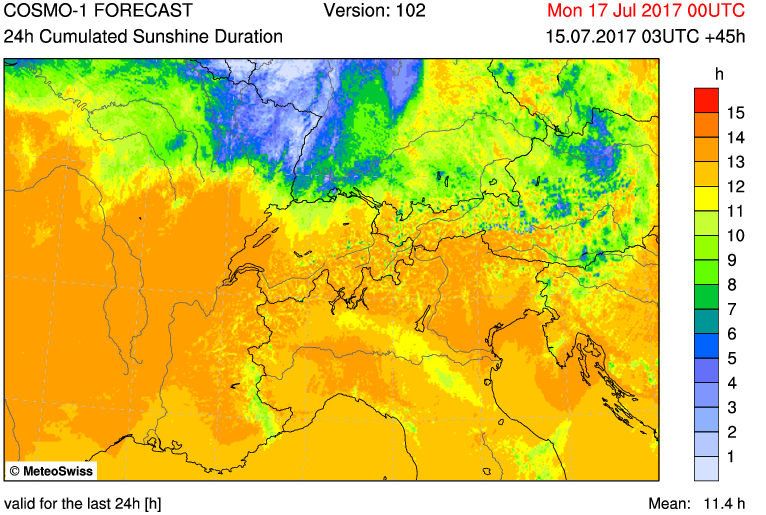
\includegraphics[width=\hsize]{klima/cosmo1.png}
\caption{COSMO-1 24-Stunden-Summe Vorhersage für Sonnenschein \cite{klima:meteoschweiz}
\label{klima:wettervorhersagen:cosmo}}
\end{figure}

\begin{itemize}
\item COSMO-1: 1158 x 774 Gitterpunkte; Maschenweite 1.1 km (0°01'); 80 vertikale Schichten; gesamter Alpenbogen mit der Schweiz im Zentrum; Zeitschrittweite 10 Sekunden; Voraussagen bis 45h, 8mal täglich; Geeignet für bessere Vorhersagen, insbesondere Gewitter, thermische Windsysteme und Föhn \cite{klima:meteoschweiz}
% Funfact, CFL = 10s / 1100m * 343 m/s = 3.12 Es scheint das Wettervorhersagen mit COSMO bereits bei einer Courant-Friedrich-Levi-Zahl von ca. 3.12 verlässlich sind. Üblich ist in numerischen Simulationen ein Wert von 1, dies würde jedoch einen 3mal höheren Rechenaufwand bedeuten.
\item COSMO-7: 393 x 338 Gitterpunkte; Maschenweite 6.6 km (0° 06'); 60 vertikale Schichten; ganz West- und Mitteleuropa; Voraussagen bis 72h, 3mal täglich \cite{klima:meteoschweiz} 
\item COSMO-E: 582 x 390 Gitterpunkte; Maschenweite 2.2 km (0° 02'); 60 vertikale Schichten; gesamter Alpenbogen mit der Schweiz im Zentrum; 21 Ensemble-Rechnungen mit leicht variierenden Initialwerten mit gleich wahrscheinlichen Vorhersagen; Geeignet für Wahrscheinlichkeitsvorhersagen von extremen Ereignissen wie Stürme oder Starkniederschläge \cite{klima:meteoschweiz} 
\end{itemize}



\subsection{Klimavorhersagen
\label{subsection:klima:entstehung}}
\rhead{Klimavorhersagen}
%%%%%%%%%%%%%%%%%%%%%%%%%%%%% In Bearbeitung%%%%%%%%%%%%%%%%%%%%%%%%%%%%%%%%

- Unterschied Wetter/Klima

- Entstehung von Klimamodellen, im wesentlichen Energiebilanzmodelle von Strahlung und Wärme, es konnten bereits Temperaturanstiege durch die zunahme von CO2 vorhergesagt werden

- Erst mit steigender Rechenkapazität wurden in den 1970er Jahren erstmals Wettervorhersagemodelle für die Klimaforschung eingesetzt. Dies bringt alle bekannten Vor- und Nachteil
 
- Allgemeine Einflussgrössen wie Einstrahlung, Fauna, zusammensetzung der Atmosphäre

- Einflussnahme durch den Menschen durch den Ausstoss zusätzlicher Treibhausgase oder auch Abholzung von Wäldern (Speicherfähigkeit von Wasser, geringe bodennahe Luftströmungen, in tropischen Wäldern verdunstet viel Wasser, somit sind diese Wälder oft für Regen in trockeneren Gebieten verantwortlich) 

- Kipppunkte im Klimasystem(Albedoeffekt) schmelzen des arktischen Eis, führt zu erhöhter aufnahme von Sonnenstrahlung durch das arktische Meer, wurde vom Eis noch reflektiert

- Auftauen des Permafrosts, in diesem ist Methan gebunden, Kanada und Russland, diese Methanmengen werden auf über das 100fache des in der heutigen Atmosphäre befindenden Methans geschätzt

- positiver Rückkopplungseffekt (Wasserdampf), je wärmer es wird desto mehr Wasser gelangt in Form von Wasserdampf in die Atmosphäre und heizen diese weiter an




\section{Spektrale Methoden
\label{section:klima:spektrale}}
\rhead{Beispiel}
Im Gegensatz zur klassischen Strömungsmechanik, welche mit Differenzmethoden arbeiten, wählen die Spektralen Methoden einen globalen Ansatz. Hierbei wird nicht mit Druck, Temperatur und weiteren Werten gerechnet sondern mit Kugel-Koeffizienten, in diesem Bezug auch als Spektral-Koeffizienten bekannt.



\subsection{Beispiel Wärmeleitungsgleichung}
Wie im vorherigen Kapitel \ref{subsection:klima:entstehung} \nameref{subsection:klima:entstehung} aufgezeigt handelt es sich bei unserer Atmosphäre um ein hochkomplexes System deren Eigenheiten bis zum heutigen Zeitpunkt noch nicht restlos verstanden sind und deshalb immer noch Teil der Forschung ist. Ein komplexes System wie das Klima kann somit unmöglich in einigen wenigen Zeilen mathematisch hergeleitet und beschrieben werden. Wir schränken uns aus diesem Grund bei den Beispielen auf ein einziges Problem, die Wärmeleitung, ein. Die Problemstellung ist einfach zu verstehen, veranschaulicht jedoch die mathematischen Schwierigkeiten und deren komplexität sehr gut.

Für die Aufgaben wird die allgemeine Wärmeleitegleichung
\begin{equation}
\frac{\partial T}{\partial t} =  \lambda \Delta T 
\label{klima:bsp:pdgl}
\end{equation}
benötigt. Die Konstante $\lambda$ beschreibt die Temperaturleitfähigkeit des Mediums.



%%%%%%%%%%%%%%%%%%%%%%%%%%%%% In Bearbeitung%%%%%%%%%%%%%%%%%%%%%%%%%%%%%%%%
\subsection{Lösung der Wärmeleitungsgleichung mit Differenzenmethoden}
Differenzenquotienten für die Zeitableitung
\begin{equation}
\varphi(x_1,x_0) = \frac{f(x_1)-f(x_0)}{x_1-x_0}
\end{equation}



Differenzenquotienten für den Laplcae


Der Laplace-Operator wird bereits verwendet~\eqref{skript:gravitation:poisson-integral}
Seite \pageref{skript:gravitation:poisson-integral}

Ich würde das alles nur in der Ebene machen, da ist es viel einfacher










\subsection{Lösung der Wärmeleitungsgleichung mit Spektralen Methoden}
Für die Spektralen Methoden werden im wesentlichen die Wärmeleitungsgleichung \eqref{klima:bsp:pdgl}
und eine Ansatzfunktion, wie die Fourier-Reihen, benötigt.
Eine Übungsaufgabe, mit der Wärmeleitegleichung auf einem Kreis, befindet sich am Ende des Kapitels \ref{skript:chapter:kugelfunktionen} \nameref{skript:chapter:kugelfunktionen} auf der Seite \pageref{skript:1101:pdgl}.

Die Fourier-Reihe auf der Kugel
\begin{equation}
T(\vartheta ,\varphi ,t)
=
a^0_0(t) + \sum_{l=1}^\infty\sum_{m=0}^l \bigl( a^m_l(t)Y^m_l(\vartheta ,\varphi)+b^m_l(t)Z^m_l(\vartheta ,\varphi)\bigr)
\label{equation:klima:fourier}
\end{equation}
wird für die Konstruktion unseres Modells benötigt. Ebenso benötigen wir zur Berechnung folgende Form des Laplace-Operators:
\begin{equation}
\Delta Y^m_l=-l(l+1)Y^m_l
\label{equation:klima:laplace}
\end{equation}

Wir müssen die Fourier-Reihe~\eqref{equation:klima:fourier} für
$T(\vartheta ,\varphi ,t)$ in die Differentialgleichung~\eqref{klima:bsp:pdgl}
einsetzen.
Dazu berechnen wir erst die Ableitungen nach $t$ und setzen die Gleichung \eqref{equation:klima:laplace} ein.
\begin{align*}
\frac{\partial T(\vartheta ,\varphi ,t)}{\partial t} &=
\dot{a}^0_0(t)+\sum_{l=1}^\infty\sum_{m=0}^l \bigl( \dot{a}^m_l(t)Y^m_l(\vartheta ,\varphi)+\dot{b}^m_l(t)Z^m_l(\vartheta ,\varphi)\bigr)
\\
\Delta T(\vartheta ,\varphi ,t) &=
\phi^c - \sum_{l=1}^\infty\sum_{m=0}^l \bigl( a^m_l(t)l(l+1)Y^m_l(\vartheta ,\varphi)+b^m_l(t)l(l+1)Z^m_l(\vartheta ,\varphi)\bigr)
\end{align*}
Die Differentialgleichung verlangt, dass diese beiden Terme übereinstimmen, also folgen die gewöhnlichen Differentialgleichungen

\begin{align*}
\dot a^0_0(t)&=\phi^c
\\
\dot a^m_l(t)&=l(l+1)a^m_l(t)&
\dot b^m_l(t)&=l(l+1)b^m_l(t)
\end{align*}
Man beachte, dass die erste Gleichung als Speziallfall in der ersten
Gleichung der zweiten Zeile enthalten ist.
\begin{align*}
a^0_0(t)&=\phi^cE+T_0
\\
a^m_l &=Ce^{-l(l+1)t}&
b^m_l &=De^{-l(l+1)t}
\end{align*}


Möchte man nun ein kleines Klimamodell daraus generieren so müssen die  $m$ und $l$ festgelegt werden, diese sind abhängig von der Komplexität welche wir haben möchte. Da wir diese klein halten wollen entscheiden wir uns für $l=1$ und $m=0$, als Praxisbezug unterteilen wir unseren Planeten in unserer Modellierung in die Nordhalbkugel und Südhalbkugel. Mit höheren $m$ und $l$ würden wir unseren Planeten in weitere Bereiche gliedern und die Modellierung komplexer gestalten, dies möchten wir nicht. Wie weitere $l$ und $m$ aussehen können wird in der Abbildund  \ref{klima:spektral:tabea} illustriert.
\begin{figure}
\centering
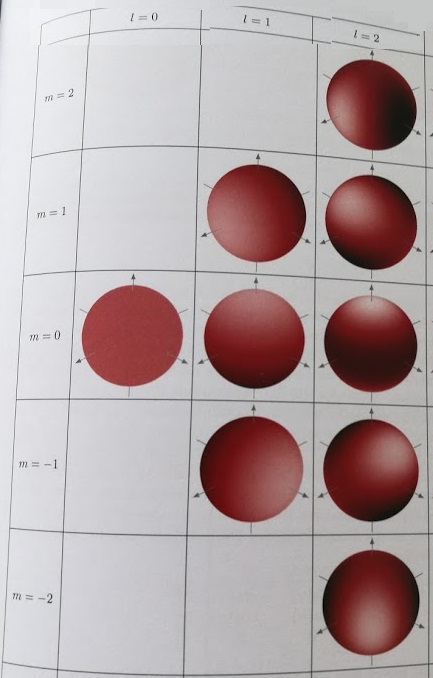
\includegraphics[width=0.7\hsize]{klima/tabeaLM.jpg}
\caption{Ich würde es als Sinvoll erachten einen solchen Ausschnitt zu präsentieren, wie sehen Sie das? \cite{skript:tabea}
\label{klima:spektral:tabea}}
\end{figure}

Die $Y^m_l$ können wir mithilfe der Formel \ref{skript:kugelfunktione:Y} lösen. Wir setzen dies in die Formel \eqref{equation:klima:fourier} ein.
\begin{align*}
T(\vartheta ,\varphi ,t)
&=
a^0_0(t) + \sum_{l=1}^\infty\sum_{m=0}^l \bigl( a^m_l(t)\frac{N^m_l}{\sqrt{2\pi}} P^m_l(\cos\vartheta)+b^m_l(t)\frac{M^m_l}{\sqrt{2\pi}} K^m_l(\cos\vartheta)\bigr)
\end{align*}
Wir berechnen den Normierungsfaktor $N^m_l$
\begin{align*}
\\
N^m_l
=
(-1)^{|m|}\sqrt{\frac{2l+1}{2}\frac{(l-|m|)!}{(l+|m|)!}}
=
(-1)^{|0|}\sqrt{\frac{2+1}{2}\frac{(1-|0|)!}{(1+|0|)!}}
=
\sqrt{\frac{3}{2}}
\end{align*}
wie auch das zugeordnete Legendre-Polynome
\begin{align*}
P^m_l(z)
=
(-1)^m(1-z^2)^{m/2}\frac{d^m}{dz^m}\frac{1}{2^ll!}\frac{d^l}{dz^l}(z^2-1)^l
=
(-1)^0(1-z^2)^{0/2}\frac{d^0}{dz^0}\frac{1}{2^1}\frac{d^1}{dz^1}(z^2-1)^1
=
\frac{(z^2-1)}{2dz}
\end{align*}

\textit{Ich glaube ich hatte hier eine Nette Idee, aber ist das überhaupt umsetzbar? Auch bin ich mir nicht sicher was die $d$ und $z$, ich dachte am Anfang an Durchmesser, Länge- oder Breitengrad. Damit scheint es aber nichts zu tun zu haben.}

\begin{align*}
T(\vartheta ,\varphi ,t)
&=
a^0_0(t) + \sum_{l=1}^\infty\sum_{m=0}^l \bigl( a^m_l(t)\frac{\sqrt{\frac{3}{2}}}{\sqrt{2\pi}} \frac{(z^2-1)}{2dz}(\cos\vartheta)+b^m_l(t)\frac{\sqrt{\frac{3}{2}}}{\sqrt{2\pi}} \frac{(z^2-1)}{2dz}(\cos\vartheta)\bigr)
\end{align*}




\subsection{Anwendung der spektralen Methoden}
- Beispiel einer äusseren Wärmequelle (das $\phi^c$) => wie einfach jetzt so ein Modell einen Anstieg der globalen Mitteltemperatur berechnet werden kann
Das $\phi^c$ beschreibt in unserem Beispiel inwiefern sich die globale Mitteltemperatur ändert. 


-Als effizientes Verfahren zur Hin- und Rücktransformation der Spektral-Koeffizienten bietet sich die schnelle Fouriertransformation (FFT) an

-Vorteile

-sphärisch harmonische Analyse zum heruasfinden der a's unb b's

-Vergleich mit klassischen Methoden

-Einflüsse wie Rückkopllungseffekte







\printbibliography[heading=subbibliography]
\end{refsection}